\chapter{Implementace}

Tato kapitola popisuje proces implementace navrhnutého řešení a uvádí použité nástroje.
Dále jsou zde obsaženy vybrané ukázky kódu a výsledné podoby systému.

\section{Rozdělení komponent}

Po analýze problému byla implementace rozdělena na dvě samostatné komponenty. Modularita
přináší jednoznačné oddělení odpovědností a zajišťuje jednodušší úpravu jednotlivých částí
díky nižší provázanosti.

\subsection{Komponenta Systém}

Komponenta Systém je součástí obrazu systému a zajišťuje začlenění výběru instalace herního serveru do prvního spuštění.
Zavádí také službu pro provoz herního serveru, která se stará o jeho spuštění po restartu systému.

\subsubsection{Příprava systému}

Pro přípravu prostředí na instalaci herního serveru byl využit mechanismus \mintinline{shell}{inithooks}, který umožňuje
spustit libovolný skript při prvním spuštění systému.
Provoz aplikace s administrátorskými oprávněními představuje v případě jejího napadení hrozbu pro systém.
Z tohoto důvodu je pro provoz herního serveru vytvořen samostatný uživatelský účet. O vytvoření uživatele se stará skript,
který dále vytvoří potřebné složky pro instalaci herního serveru.

\subsubsection{Výběr herního serveru}

Po vytvoření uživatele a prvotním nastavení systému je nutné provést výběr herního serveru.
Pokud uživatel při vytváření instance systému zadal inicializační skript s potřebnými daty, vytvořený skript tato
data načte a podle proměnné \mintinline{shell}{GAME} zvolí herní server.

V případě interaktivního přístupu bez inicializačního skriptu dojde ke stažení repozitáře s Komponentou Herní server,
ze kterého je získán seznam aktuálně podporovaných her. Tento seznam tudíž není pevně daný v obrazu systému a je možné
přidávat podporu nových serverů bez nutnosti vytvoření nového obrazu.
Následně skript zobrazí okno výběru herního serveru pomocí knihovny \mintinline{shell}{pythondialog}, kterou využívá mechanismus
\mintinline{shell}{inithooks}. Z pohledu uživatele se tak jedná o graficky navazující, jednolitý systém. Příklad tohoho výběru
je možné vidět na obrázku \ref{fig:game-selection} v sekci Ukázky.

Pokud došlo ke spuštění systému bez interaktivního prostředí a uživatel nezadal inicializační skript, nástroj \mintinline{shell}{inithooks} vyplní
potřebná data náhodnými hodnotami. Po prvním přihlášení pomocí SSH dojde k automatickému spuštění interaktivní inicializace systému.
Uživatel může vybrat požadovaný herní server během této inicializace nebo později pomocí konfigurační konzole systému.

\subsubsection{Instalace herního serveru}

Instalace a konfigurace herního serveru je dále uskutečněna pomocí stažené Komponenty Herní server. Tento proces bude popsán v části věnované dané komponentě.

\subsubsection{Systémová služba}

Pro zajištění automatického běhu herního serveru po spuštění systému je zavedena systémová služba, která zajišťuje správné spouštění
a ukončování herního serveru.

\subsection{Komponenta Herní server}

Komponenta Herní server slouží k automatické instalaci a nastavení herních serverů. Tato komponenta je zcela nezávislá na
vybraném operačním systému a je tedy možné ji využít pro instalaci herního serveru v dalších distribucích Linuxu.
Využívá správce herních serverů LinuxGSM, který umožňuje servery automaticky stahovat a instalovat.

\subsubsection{Instalace herního serveru}

Před instalací vybraného herního serveru provede vytvořený skript instalaci nejčastěji využívaných balíčků pro provoz serverů.
Pomocí argumentů při spouštění skriptu lze kromě herního serveru nastavit i požadované umístění herního serveru a účet, pomocí kterého
se bude herní server spouštět. Pro zvýšení bezpečnosti není povoleno přiřadit herní server účtu `root`.

Následně dojde ke stažení správce LinuxGSM a jeho spuštění za účelem instalace herního serveru. LinuxGSM podporuje automatickou instalaci
potřebných balíčků pro provoz serveru, po stažení a instalaci je tedy herní server připraven ke spuštění.

\subsubsection{Nastavení herního serveru}

Komponenta podporuje volitelné spuštění skriptů před a po instalaci serveru. Tyto skripty slouží
ke specifické konfiguraci systému a k následnému nastavení herního serveru před jeho spuštěním.
Údaje pro nastavení herního serveru lze předat pomocí předem nastavených proměnných v příkazové řádce. V případě absence těchto údajů
je uživatel vyzván k jejich doplnění v průběhu instalace.

\section{Nástroje}

\subsection{Editor}

Pro vývoj kódu byl použit editor Visual Studio Code \cite{vscode}, který umožňuje snadnou integraci s verzovacím systémem
a podporuje množství typů souborů. Pomocí rozšiřujících doplňků je možné doplnit editor o pokročilé funkce či podporuj
dalších programovacích jazyků.

\subsection{Verzování}

K verzování projektu byl využit verzovací nástroj Git \cite{git}. Tento volně dostupný nástroj nabízí
neomezené distribuované verzování a je vhodný pro správu kódu.
Kód byl pomocí nástroje ukládán na webový server GitHub, který využívají i používané systémy TurnKey GNU/Linux
a LinuxGSM.

\subsection{Prostředí pro tvorbu obrazu}

Pro sestavení obrazu byl využit operační systém TKLDev \cite{tkldev}, provozovaný jako lokální virtuální stroj. Tento systém, spravovaný vývojáři TurnKey GNU/Linux,
je určen pro tvorbu nových obrazů této distribuce s přednastavenou aplikací. Umožňuje vytvářet instalační obrazy systémů a podporuje
také tvorbu obrazů určených k provozu u poskytovatelů cloudových služeb.

\section{Ukázky}

\subsection{Spuštění instance systému}

Ukázka \ref{fig:openstack} zobrazuje proces spouštění nové instance systému v cloudovém prostředí OpenStack \cite{openstack}.
Uživatel pomocí průvodce přidělí systémové prostředky a zvolí požadovanou konfiguraci systému.
Průvodce nabízí uživateli možnost vložit skript, který nastaví potřebná data pro inicializaci a umožní automatickou instalaci herního serveru. 

\begin{figure}[h]
    \centering
    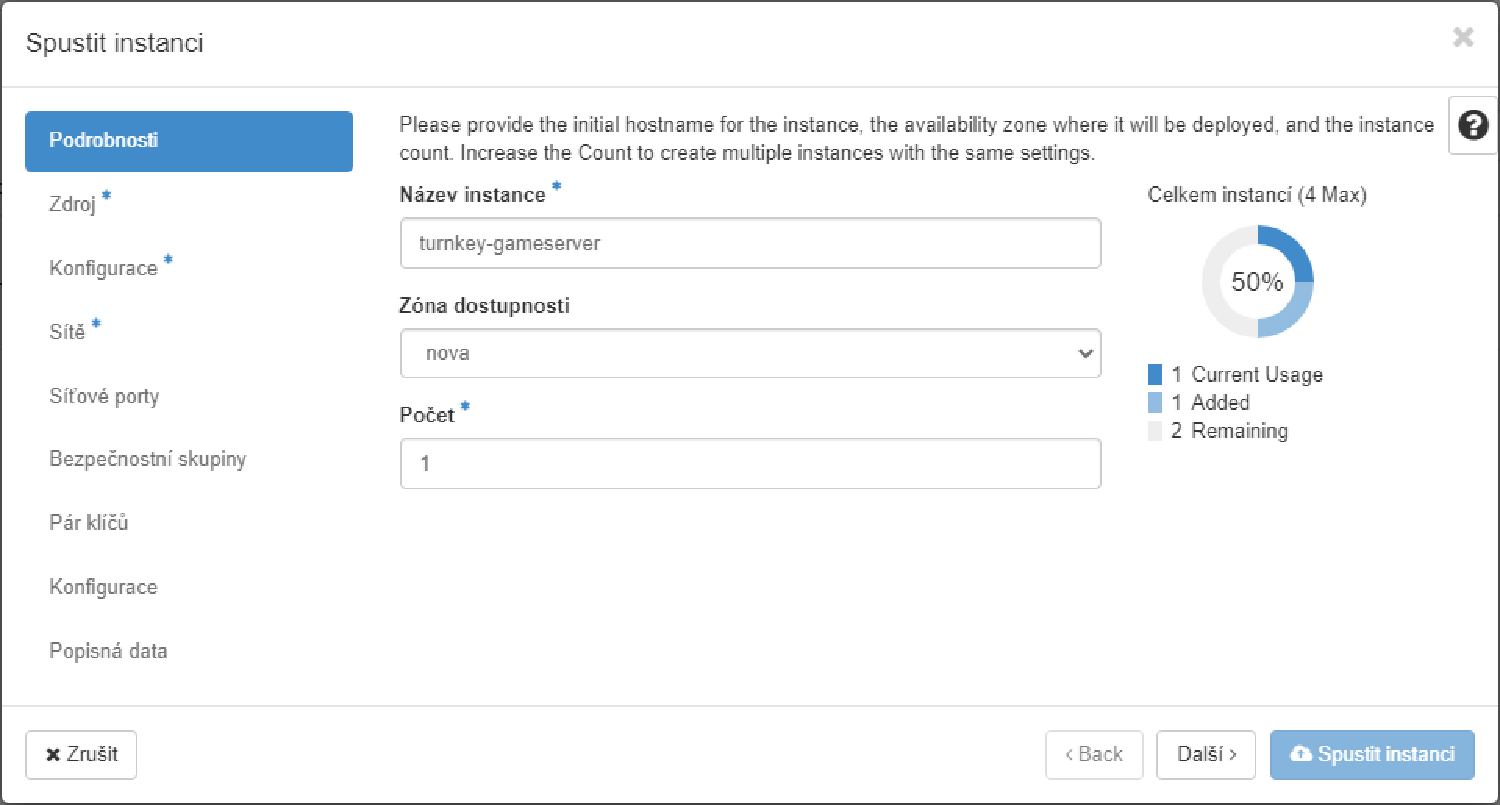
\includegraphics[width=1\linewidth]{chapters/images/openstack.pdf}
    \caption{Spuštění systému v prostředí OpenStack \cite{openstack}}
    \label{fig:openstack}
\end{figure}

\subsection{Interaktivní výběr herního serveru}

Na obrázku \ref{fig:game-selection} je zobrazen interaktivní výběr herního serveru. Tento výběr je automaticky
k dispozici při prvním spuštění systému, pokud uživatel neurčil herní server pomocí inicializačního skriptu.

\begin{figure}[h]
    \centering
    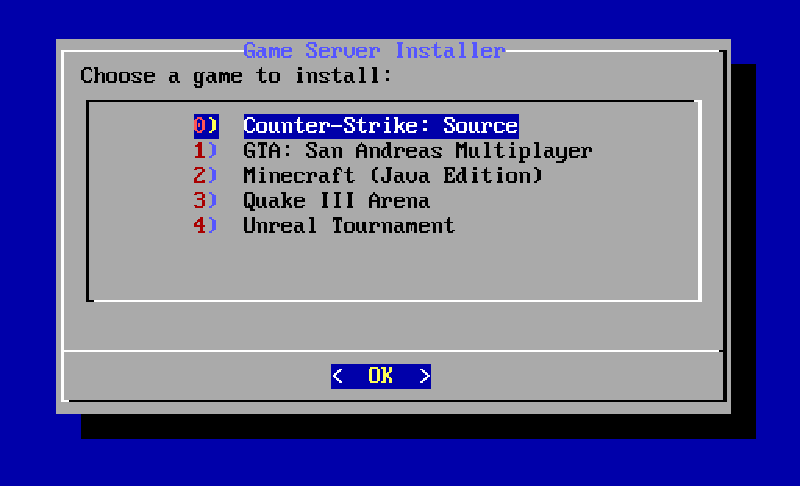
\includegraphics[width=1\linewidth]{chapters/images/game-selection.pdf}
    \caption{Interaktivní výběr hry při prvním spuštění}
    \label{fig:game-selection}
\end{figure}

\subsection{Automatický výběr herního serveru}

V případě plně automatického nasazení herního serveru je nutné použít inicializační skript, který před prvním spuštěním systému
zapíše do souboru \mintinline{shell}{/etc/inithooks.conf} potřebná data pro automatickou konfiguraci systému.
V ukázce \ref{code:init-script} je uveden inicializační skript, pomocí kterého dojde k instalaci herního serveru pro hru \mintinline{shell}{GTA: San Andreas Multiplayer}
včetně nastavení administrátora serveru.

\begin{listing}[h!]
    \caption{Ukázkový inicializační skript}
    \label{code:init-script}
    \begin{minted}{shell}
#!/bin/bash

cat>/etc/inithooks.conf<<EOF
export ROOT_PASS=SecretRootPassword
export DB_PASS=SecretMysqlPassword
export APP_PASS=SecretGameuserPassword
export APP_EMAIL=admin@example.com
export HUB_APIKEY=SKIP
export SEC_UPDATES=FORCE

export GAME=samp
export GAME_RCON_PASS=GameserverAdminPassword
EOF
    \end{minted}
\end{listing}

\subsection{Přidání nové hry}

Ukázky kódu \ref{code:game-props-script} a \ref{code:game-config-script} demonstrují přidání podpory pro nový herní server. Jedná se o dva skripty komponenty Herní server,
které zavádějí podporu pro server hry \mintinline{shell}{Minecraft} a umožňují jeho minimální počáteční konfiguraci.
Skript \mintinline{shell}{game_properties.sh} zavádí proměnné, které jsou instalačním programem využity k identifikaci herního serveru.
Druhý skript poté umožňuje nastavit uživatelské jméno administrátora serveru pomocí předdefinované proměnné, případně interaktivně.

\begin{listing}[h]
    \caption{Skript \mintinline{shell}{game_properties.sh}}
    \label{code:game-props-script}
    \begin{minted}{shell}
GAME="mc"
GAME_LONG_NAME="Minecraft (Java Edition)"
    \end{minted}
\end{listing}

\begin{listing}[h]
    \caption{Skript \mintinline{shell}{post_install.sh}}
    \label{code:game-config-script}
    \begin{minted}{shell}
#!/bin/bash

# Set server admin
if [ -z "$GAME_ADMIN" ]; then
    read -p "Server admin username: " GAME_ADMIN || GAME_ADMIN=''
    echo
fi
run_as_user "echo \"$GAME_ADMIN\" > \"$GAMEDIR/serverfiles/ops.txt\""
    \end{minted}
\end{listing}


\section{Možnosti rozšíření}

Systém v současné době podporuje pouze čtyři herní tituly. Díky decentralizovanému návrhu
a osamostatnění části pro správu herních serverů od operačního systému je však možné doplňovat podporu
pro další herní servery bez zásahu do obrazu systému.

Některé herní servery vyžadují před spuštěním přihlášení k platformě Steam za účelem ověření zakoupení licence
pro jejich provoz. Tyto servery nejsou v současné chvíli systémem podporovány. V případě jejich podpory
by bylo nutné získat od uživatele jeho přihlašovací údaje, pomocí kterých by bylo možné licenci ověřit.

Systém je díky možnosti plně automatického spuštění vhodný i pro provoz v komerčním prostředí, vzhledem k aktuálnímu
množství podporovaných her ale není konkurenceschopný.
